\section{Directed Simplex Memory Graph}
\label{sec:directed_graph}

The lattice $V_{n,m}$ defined in \cref{sec:preliminaries} provides only the set of hidden nodes. To obtain a functional architecture, we must specify how these nodes are connected and how information flows through the network. This section constructs the directed hidden graph that defines the simplex memory network.

The construction proceeds in two steps. First, we connect lattice points that are nearest neighbors, yielding an undirected graph that captures the local geometry of the simplex. Second, we orient these edges using a linear potential function that encodes the desired direction of information flow---from the input facet toward the output facet. The resulting directed graph is acyclic and exhibits a natural layer structure with geometrically induced skip connections.

We begin with the undirected connectivity.

\begin{definition}[Nearest neighbors]
Two nodes $\alpha,\alpha'\in V_{n,m}$ are nearest neighbors if and only if
\[
\alpha' = \alpha + e_i - e_j
\]
for some $i\neq j$ with $\alpha_j\geq 1$. Equivalently, $\alpha'$ is obtained from $\alpha$ by moving one unit of barycentric mass from the $j$th coordinate to the $i$th coordinate.
\end{definition}

All such edges have the same Euclidean length in the ambient simplex:
\[
\|x(\alpha')-x(\alpha)\| = \frac{1}{m-1}\|e_i-e_j\| = \frac{\sqrt{2}}{m-1}.
\]
Thus the lattice induces a regular grid in which every node has a uniform local neighborhood structure.

However, the undirected graph alone does not specify a direction of information flow. To obtain a feedforward architecture, we must orient these edges. The orientation is determined by assigning potentials to the vertices of the simplex and extending linearly to the lattice.

\begin{definition}[Vertex potentials and induced orientation]
Assign the vertex potentials
\[
\beta_a=0,
\qquad
\beta_b=2,
\qquad
\beta_{c_1}=\cdots=\beta_{c_{n-1}}=1.
\]
Equivalently, $\beta_0=0$, $\beta_1=2$, and $\beta_2=\cdots=\beta_n=1$. The hidden potential $H: V_{n,m} \to \R$ is defined by
\[
H(\alpha) := \sum_{k=0}^n \beta_k\alpha_k = 2\alpha_1 + \alpha_2 + \cdots + \alpha_n.
\]
A directed edge is retained from $\alpha$ to $\alpha' = \alpha + e_i - e_j$ if and only if
\[
\alpha_j\geq 1
\qquad\text{and}\qquad
\beta_i > \beta_j.
\]
Edges with $\beta_i=\beta_j$ are deleted.
\end{definition}

\begin{figure}[ht]
\centering
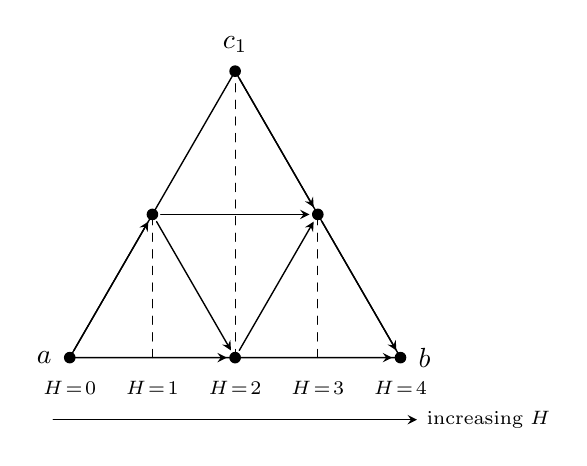
\begin{tikzpicture}[scale=1.05, >=stealth, line width=0.5pt,
                    line cap=round, line join=round]
  % n=2, m=3 equilateral triangle: a=(0,0), b=(4,0), c_1=(2,2sqrt3)
  % Key fact: H(alpha) = 2*alpha_1 + alpha_2 = x-coordinate of the node.
  % Isopotential lines are therefore vertical.
  \coordinate (a)  at (0,    0    );  % (2,0,0)  H=0
  \coordinate (P1) at (1,    1.732);  % (1,0,1)  H=1
  \coordinate (P2) at (2,    0    );  % (1,1,0)  H=2
  \coordinate (c1) at (2,    3.464);  % (0,0,2)  H=2
  \coordinate (P3) at (3,    1.732);  % (0,1,1)  H=3
  \coordinate (b)  at (4,    0    );  % (0,2,0)  H=4

  % Isopotential lines: x=H (vertical dashed)
  \draw[dashed, line width=0.4pt] (1,0) -- (1,1.732);  % H=1
  \draw[dashed, line width=0.4pt] (2,0) -- (2,3.464);  % H=2 (full height to c_1)
  \draw[dashed, line width=0.4pt] (3,0) -- (3,1.732);  % H=3

  % Triangle boundary
  \draw (a) -- (b) -- (c1) -- cycle;

  % ---- Directed edges ----
  % DeltaH = 1 (straight arrows)
  \draw[->, shorten <=3pt, shorten >=3pt] (a)  -- (P1);
  \draw[->, shorten <=3pt, shorten >=3pt] (P1) -- (P2);
  \draw[->, shorten <=3pt, shorten >=3pt] (P2) -- (P3);
  \draw[->, shorten <=3pt, shorten >=3pt] (c1) -- (P3);
  \draw[->, shorten <=3pt, shorten >=3pt] (P3) -- (b);
  % DeltaH = 2 (skip connections, straight)
  \draw[->, shorten <=3pt, shorten >=3pt] (a)  -- (P2);
  \draw[->, shorten <=3pt, shorten >=3pt] (P1) -- (P3);
  \draw[->, shorten <=3pt, shorten >=3pt] (P2) -- (b);

  % ---- Nodes ----
  \foreach \p in {a, b, c1, P1, P2, P3} \fill (\p) circle (2pt);

  % ---- Vertex / node labels ----
  \node[left=3pt]        at (a)  {$a$};
  \node[right=3pt]       at (b)  {$b$};
  \node[above=3pt]       at (c1) {$c_1$};

  % H-value ticks along the bottom
  \foreach \x/\hv in {0/0, 1/1, 2/2, 3/3, 4/4}
    \node[below=5pt, font=\scriptsize] at (\x,0) {$H\!=\!\hv$};

  % Gradient arrow
  \draw[->] (-0.2,-0.75) -- (4.2,-0.75)
      node[right, font=\scriptsize] {increasing $H$};
\end{tikzpicture}
\caption{Potential flow on $\mathrm{SMN}(2,3)$ ($n=2$, $m=3$).
  Each node $\alpha\in V_{2,3}$ is shown at its geometric position in
  the equilateral triangle; its potential $H(\alpha)=2\alpha_1+\alpha_2$
  equals its horizontal coordinate.
  Vertical dashed lines are isopotential sets.
  Solid arrows are $\Delta H=1$ edges; bent arrows are $\Delta H=2$
  skip connections.  All edges point strictly rightward.}
\label{fig:potential-flow}
\end{figure}

This orientation rule has a simple interpretation: information flows from lower-potential vertices to higher-potential vertices. The admissible edge types are therefore exactly
\[
a\to c_k,\qquad c_k\to b,\qquad a\to b,
\qquad k=1,\dots,n-1,
\]
while all edges among the intermediate vertices $c_1,\dots,c_{n-1}$ are removed. Geometrically, this reflects the flow from the input vertex $a$ (potential 0) through the intermediate layer (potential 1) to the output vertex $b$ (potential 2), together with a direct skip connection from $a$ to $b$.

The potential-based orientation immediately implies acyclicity.

\begin{proposition}[Acyclicity]
The directed hidden graph $(V_{n,m},E^{\rightarrow}_{n,m})$ is acyclic.
\end{proposition}

\begin{proof}
If $\alpha' = \alpha + e_i-e_j$ is a retained directed edge, then $H(\alpha')-H(\alpha)=\beta_i-\beta_j > 0$. Hence the potential strictly increases along every directed edge. A directed cycle would force the potential to strictly increase and return to its initial value, which is impossible.
\end{proof}

We can now give the formal definition of the architecture.

\begin{definition}[Simplex memory network]
For integers $n\geq 2$ and $m\geq 2$, the \emph{simplex memory network} $\SMN(n,m)$ is the directed hidden graph together with its distinguished input and output interfaces:
\[
\SMN(n,m)
:=
\bigl(V_{n,m}, E^{\rightarrow}_{n,m}, F_{\mathrm{in}}, F_{\mathrm{out}}\bigr).
\]
\end{definition}

Having defined the directed graph, we now compute its basic combinatorial properties. These quantities determine the architectural capacity and computational cost.

\begin{proposition}[Directed edge count]
The directed hidden edge set satisfies
\[
\card{E^{\rightarrow}_{n,m}} = (2n-1)\binom{m+n-2}{n}.
\]
\end{proposition}

\begin{proof}
There are $2n-1$ admissible directed edge types:
\[
a\to c_1,\dots,a\to c_{n-1},\qquad c_1\to b,\dots,c_{n-1}\to b,\qquad a\to b.
\]
Consider one such type, say $a\to c_k$, corresponding to the move $\alpha \mapsto \alpha + e_{k+1}-e_0$ with $\alpha_0\geq 1$. Setting $\alpha_0' := \alpha_0-1\geq 0$, we obtain
\[
\alpha_0' + \alpha_1 + \cdots + \alpha_n = m-2,
\]
whose number of nonnegative solutions is $\binom{m+n-2}{n}$. The same count holds for every admissible edge type, and the result follows.
\end{proof}

The edge count formula reveals the scaling behavior of the architecture. The factor $(2n-1)$ counts the number of directed edge types emanating from each source node, while the binomial coefficient counts how many such source nodes exist in the lattice. This combinatorial structure will be important when we analyze the forward and backward propagation laws in Section 5.
